\begin{figure}[h]
    \centering
    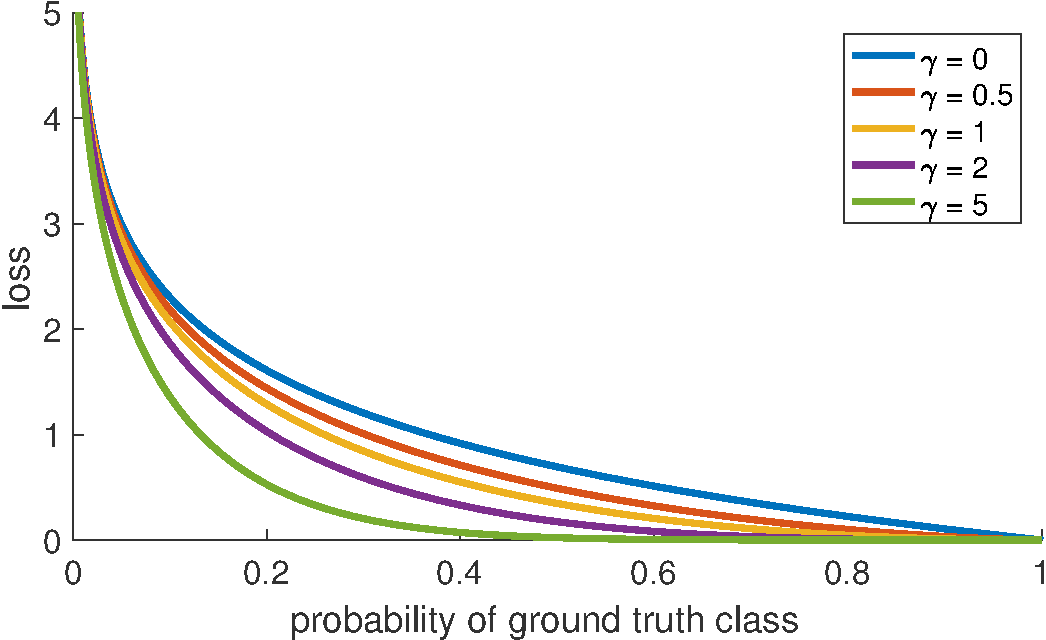
\includegraphics[width=0.55\linewidth]{images/focal-loss.pdf}
    \caption{Focal loss at different $\gamma$ values \cite{lin2018focalloss}. When $\gamma=0$, it is equivalent to cross-entropy loss. As $\gamma$ increases, the loss focuses more on hard examples, down-weighting easy ones.}
    \label{fig:focal-loss}
\end{figure}
